\section{Projekt}

Projekt zostanie zaimplementowany w języku programowania Python. 
Główny program będzie  realizował kolejne zadania (TASKi) umieszczone w kolejce zadań. 
Określenie zadań 
Schemat realizacji programu będzie zapisany w pliku XML (plik konfiguracyjny). Takie rozwiązanie problemu umożliwi łatwą edytowalność workflowu bez konieczności zmian w implementacji programu. Dokładny opis wejścia zostanie określony w trakcie realizacji projektu.
Opis eksperymentu znajdować się będzie w zestawie plików CSV, który w dalszej części pracy nazywamy MAP PLATEm. 


Podstawowy schemat działania programu zgodny z opisem \ref{sec:workflow} jest przedstawiona na schemacie \ref{fig:workflow}. Program na podstawie pliku wejściowego będzie sprawdzał, czy pod danym adresem znajduje się folder z przeanalizowanym dołkiem. Jeżeli tak to zostanie on skopiowany i odpowiednie zadanie opisujące procedurę analizy danego dołka zostanie dodane do kolejki zadań. Zadania z kolejki zadań będą równolegle obsługiwane przez zdefiniowaną liczbę podprocesów. Liczba ta również zostanie określona w pliku konfiguracyjnym. Liczba tych podprocesów musi być określona w ten sposób, aby ich wielość nie doprowadziła do przeciążenia zasobów komputera.
Postawowa analiza jest zakończona, gdy wsyzstkie foldery z obrazowaniem dołków zostaną przesłane i poddane analizie.
 
\begin{figure}[htp]
  \begin{center}
    \includegraphics[width=0.8\linewidth]{resources/img/Workflow.pdf}
  \caption{Podstawowa ścieżka działania programu.  } 
  \label{fig:workflow}
  \end{center}
\end{figure}

\subsection{Moduły i funckonalności}

Ze względu na chęć wykorzystania poszczególnych funkcjonalności w innych projektach założeniem projektowym jest stworzenie programu możliwie, jak najbardziej modularnego z oddzielnym niezależnym interfacem. Główne moduły programu są zaprezentowane na schemacie \ref{fig:modules}.
Poniżej znajduje się ich szczegółowy opis.

\begin{figure}[htp]
  \begin{center}
    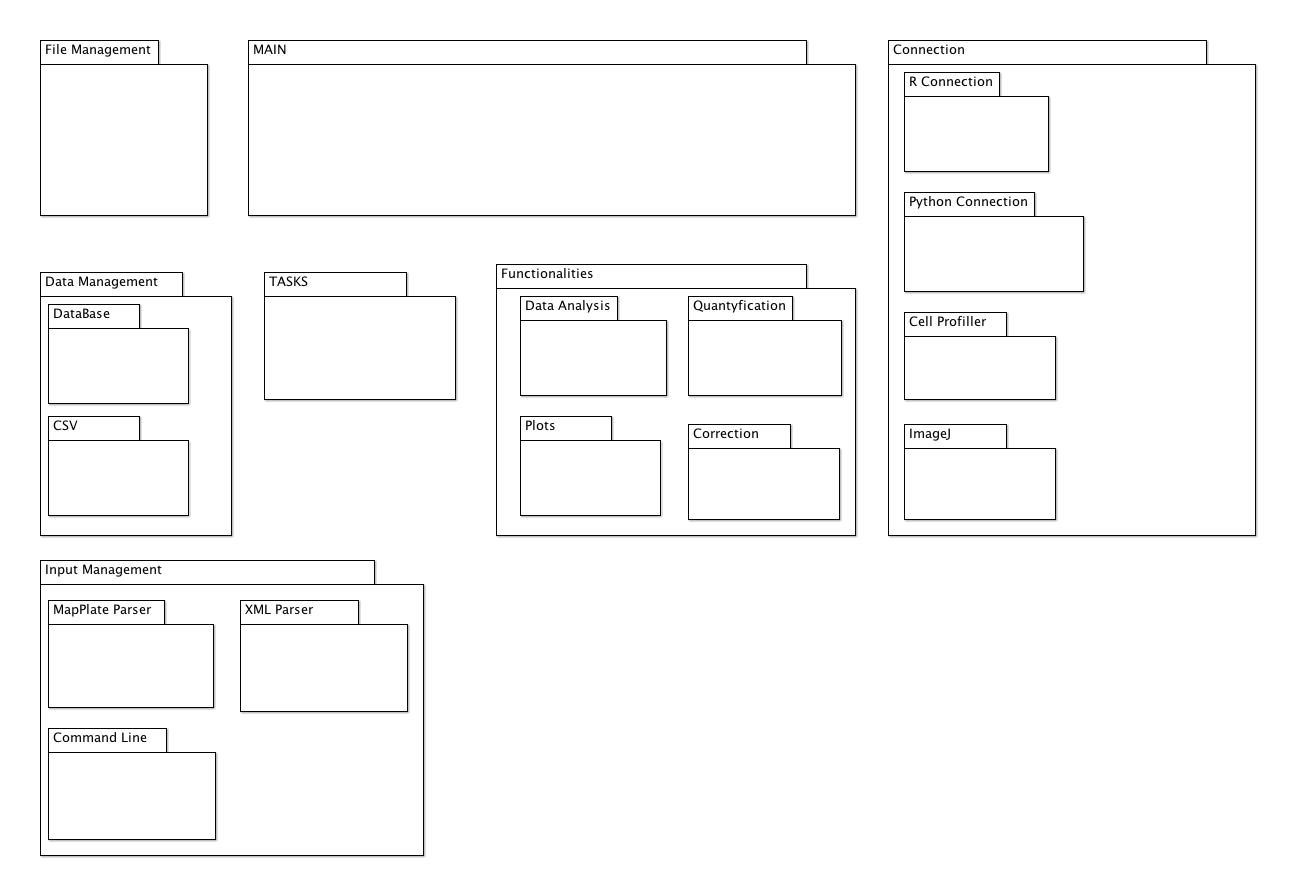
\includegraphics[width=0.8\linewidth]{resources/img/Modules.png}
  \caption{Schemat prezentujący główne moduły funkcjonalne oprogramowania..} 
  \label{fig:modules}
  \end{center}
\end{figure}

\begin{itemize}
\item Main - silnik programu zarządzający całym oprogramowaniem. Moduł wczytuje wejście do programu oraz wywołuje odpowiedni moduł do jego parsowania, a następnie wczytuje i wywołuje kolejne zadania z kolejki zadań.
\item Tasks - moduł zawierający reprezentację kolejnych kroków programu, jak i ich obsługę.Moduł posiada reprezentację w paradygmacie obiektowym.
Poszczególne zadania są reprezentowane, jako obiekty  zdefiniowanych klas dziedziczących po interefejsie TASK. 
Każdy z modułów funkcjonalnych programu oraz każda powtarzalna grupa funkcjonalności będzie miała przypisaną odpowiednią klasę.
Obiekt klasy dziedziczącej po interfejsie TASK wywoływany jest za pomocą funkcji execute wraz ze słownikiem wejściowym, który zawiera wszystkie dane programu. Funkcja execute zwraca zmodyfikowany przez obiekt słownik.
Wywołanie funkcji execute na obiekcie odpowiedniej podklasy interfejsu TASK powoduje wywołanie z odpowiednim wejściem funkcji z przypisanych modułów funkcjonalnych.

I tak na przykład, gdy będziemy chcieli wywołać odpowiednią funkcję, które wizualizuje dane w programie R będziemy musieli wywołać obiekt klasy TASK R, który będzie posiadał nazwę tej funckji, zdefiniowane wejście oraz zbiór danych do analizy.

\begin{figure}[htp]
  \begin{center}
    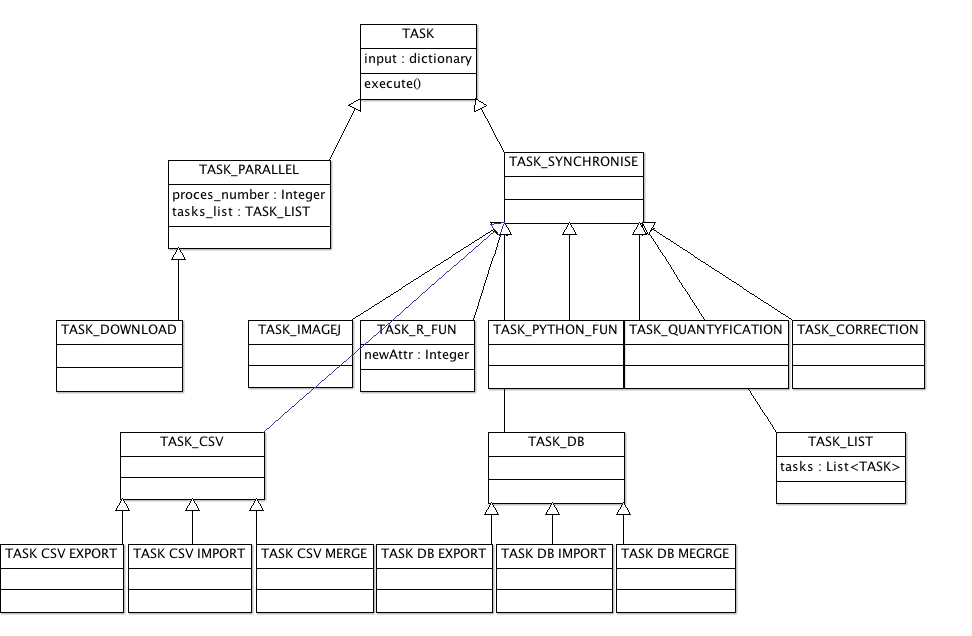
\includegraphics[width=0.8\linewidth]{resources/img/Tasks.png}
  \caption{Diagram klas występujących w module Task, będących instancją realizowanych w projekcie zadań.} 
  \label{fig:modules}
  \end{center}
\end{figure}

\begin{itemize}
\item TASK PARALLEL - specjalna implementacja interfejsu TASK, która umożliwia równoległe (ze względu na input) wykonanie zadań zapisanych w obiekcie klasy TASK LIST. Przykładem jest podklasa TASK DOWNLOAD, która będzie implementowała pobieranie danych eksperymentalnych i równoległe do niego wykonywanie kwantyfikacji oraz korekty danych.
\item TASK SYNCHRONISE - podinterefejs interfejsu  TASK, którego implementacje będą wykonywały synchronicznie zapisane w nich zadania.
\item TASK LIST - Specjalna implementacja interfejsu TASK, który zawiera listę zadań wykonywanych synchronicznie.
\end{itemize}

Podstawowy schemat konfiguracyjny będzie wyglądał :
\begin{enumerate}
\item TASK DOWNLOAD - 
\begin{itemize}
\item pobranie eksperymentu referencyjnego
\item zdefiniowaną ścieżka do folderu wejściowego oraz wyjściowego,
\item TASK LIST
\begin{itemize}
\item TASK QUANTYFICATION 
\begin{itemize}
\item zdefiniowany algorytm kwantyfikacji
\end{itemize}
\end{itemize}
\end{itemize}
\item TASK DOWNLOAD - 
\begin{itemize}
\item pobranie eksperymentu 
\item zdefiniowaną ścieżka do folderu wejściowego oraz wyjściowego,
\item TASK LIST
\begin{itemize}
\item TASK CORRECTION
\item TASK QUANTYFICATION
\item TASK DATA ANALYSIS
\end{itemize}
\end{itemize}
\item TASK CSV MERGE
\item TASK DATA ANALYSIS
\item TASK R FUN 
\begin{itemize}
\item Wizualizacja wyników
\end{itemize}
\item TASK IMAGE J
\item TASK CSV EXPORT
\end{enumerate}

Dokładne określenie liczby oraz funkcjonalności poszczególnych zadań zostanie określone w trakcie trwania projektu.

\item File Management - moduł służący do zarządzania plikami (np.: kopiowanie, usuwanie plików)
\item Data Management - moduł służący do zarządzania, importowania i eksportowania danych do różnych formatów.
\item Input Management - moduł służacy do parsowania wejścia do programu. Jako wejście do programu rozumiemy plik konfiguracyjny w formacie XML opisujący schemat działania programu oraz MAP PLATE opisujący ekpseryment.
\item Functionalities - moduł zawierający implementację poszczególnych funcjonlności oprogramowania (np. kwantyfikacja, analiza danych, itp.).
\item Connection - moduł implementujący funkcje umożliwiające wywoływanie oddzielnych i niezlaeżnych skrytptów, bądź zewnętrznych programów. Wynika to z tego, że projekt zakłada wykorzystanie różnego oprogramowania zewnętrzengo np.:  do analizy obrazów, statystycznej analizy oraz wizualizacji danych eksperymentalnych. Moduł Connection ma służyć do wywoływania skryptów w poszczególnych językach programowania, bądź programach. W przyszłości podmoduły z modułu Connection mają zostać wykorzystane do rozszerzenia  programu Cell Profiller.
Zakładamy powstanie następujących modułów :
\begin{itemize}
\item python -  statystyczna analiza danych,
\item pakiet R - statystyczna analiza oraz wizualizacja danych,
\item Cell Profiller - analiza obrazów i kwantyfikacja eksperymentów,
\item Image J - edytowanie i korekta obrazów, zbiorcza wizualizacja eksperymentów.
\end{itemize}
\end{itemize}


\subsection{Zarządzanie projektem}
W celu sprawnego zarządzania projektem wykorzystamy podstawowe techniki występujące w tworzeniu oprogramowania.
\begin{itemize}
\item System kontroli wersji - git, github.
\item Kontorla jakości kodu - np. zastosowanie pakietu do tworzenia logów.
\item Dokumnetacja każdego modułu dołączona w osobnych plikach wewnątrz proejktu. Automatyczne pliki konfiguracyjne. Przykłady zastosowania.
\item Planowanie projektu :
\begin{itemize}
\item Długoterminowe - rozpisany plan pracy w okresie 6 miesięcznym,
\item Krótkoterminowe - lista zadań na okres 2 tygodni (Google Keeps).
\end{itemize}
\item Spotkania cotygodniowe.
\end{itemize}

